\documentclass[twocolumn,10pt]{article}

\usepackage[utf8]{inputenc}
\usepackage[T1]{fontenc}
\usepackage{amsmath,amssymb,amsthm}
\usepackage{mathtools}
\usepackage{geometry}
\usepackage{graphicx}
\usepackage{float}
\usepackage{booktabs}
\usepackage{array}
\usepackage{hyperref}
\usepackage{cleveref}
\usepackage{algorithm}
\usepackage{algpseudocode}
\usepackage{listings}
\usepackage{xcolor}
\usepackage{tikz}
\usetikzlibrary{arrows.meta,positioning,calc,shapes}

\geometry{margin=0.75in}

% Theorem environments
\newtheorem{theorem}{Theorem}[section]
\newtheorem{lemma}[theorem]{Lemma}
\newtheorem{corollary}[theorem]{Corollary}
\newtheorem{definition}[theorem]{Definition}
\newtheorem{proposition}[theorem]{Proposition}
\newtheorem{axiom}[theorem]{Axiom}
\newtheorem{principle}[theorem]{Principle}

\theoremstyle{remark}
\newtheorem{remark}[theorem]{Remark}
\newtheorem{example}[theorem]{Example}

% Custom commands
\newcommand{\Sk}{S_k}
\newcommand{\St}{S_t}
\newcommand{\Se}{S_e}
\newcommand{\Sspace}{\mathcal{S}}
\newcommand{\Scoord}{\mathbf{S}}
\newcommand{\eps}{\varepsilon}
\newcommand{\Gres}{\mathcal{G}}
\newcommand{\tmark}{\mathsf{t}}
\newcommand{\trmark}{\mathsf{T}}

% Code listing style
\lstdefinelanguage{Trajectory}{
  keywords={system, completion, navigate, partition, phase_lock, morphism, catalyst, project, complete, compose, when, from, to, via, where, constraint, entity, relation, infer, derive, observe},
  keywordstyle=\color{blue}\bfseries,
  keywords=[2]{Int, Real, Trit, Tryte, Partition, Category, Trajectory, PhaseLock, Morphism, Completion},
  keywordstyle=[2]\color{purple},
  comment=[l]{//},
  commentstyle=\color{gray}\itshape,
  stringstyle=\color{red},
  morestring=[b]",
  sensitive=true,
}

\lstset{
  language=Trajectory,
  basicstyle=\ttfamily\scriptsize,
  breaklines=true,
  frame=single,
  xleftmargin=2mm,
  framexleftmargin=2mm,
}

\title{\textbf{Trajectory Computing: A Post-Explanatory Programming Paradigm Based on Categorical Completion in Bounded Phase Space}}

\author{
Kundai Farai Sachikonye\\
\texttt{kundai.sachikonye@wzw.tum.de}
}

\date{\today}

\begin{document}

\maketitle

\begin{abstract}
We present Trajectory Computing, a programming paradigm in which computation is trajectory completion in bounded S-entropy phase space rather than sequential instruction execution. The paradigm rests on three foundational principles: (1) the triple equivalence of oscillation, category, and partition; (2) the identity of trajectory and position in ternary representation; and (3) the equivalence of computing and verification at the $\eps$-boundary.

Programs specify \textit{completion conditions}---categorical structures defining what solutions look like---rather than algorithms specifying how to find them. The runtime navigates S-entropy space $\Sspace = [0,1]^3$ to the $\eps$-boundary, one categorical step from closure, which represents maximum possible knowledge given the Gödelian residue $\Gres$ inherent in any bounded formal system.

We establish that this approach inverts the traditional computational model: instead of assuming initial conditions and simulating forward, Trajectory Computing specifies the completion point and derives what the trajectory (and hence initial conditions) must have been. Since trajectory and position are identical in ternary encoding, and computing reaches the same $\eps$-boundary as verification, the solution simultaneously encodes its own proof.

We present the complete syntax and semantics of the Trajectory language, its type system based on partition coordinates $(n, \ell, m, s)$, the architecture of the categorical runtime, and implementation strategies exploiting the $3^k$ hierarchical structure. Examples demonstrate applications to physics derivation, constraint satisfaction, and semantic processing. The paradigm achieves $O(\log n)$ navigation complexity through recursive structure exploitation and eliminates the von Neumann separation between processor and memory through categorical identity unification.

\textbf{Keywords:} trajectory computing, categorical completion, S-entropy navigation, ternary representation, post-explanatory epistemology, Gödelian residue, $\eps$-boundary, partition coordinates
\end{abstract}

%==============================================================================
\section{Introduction}
\label{sec:introduction}
%==============================================================================

Contemporary programming paradigms---imperative, functional, object-oriented, logic-based---share a common assumption: computation proceeds from known initial conditions through specified operations to produce results. The program encodes \textit{how} to transform input into output. This forward-simulation model, inherited from the von Neumann architecture \cite{vonneumann1945first} and formalized in Turing machine computation \cite{turing1936computable}, has proven extraordinarily successful but embeds a fundamental epistemological assumption that we challenge.

The assumption is this: initial conditions are knowable. Given complete specification of the starting state, deterministic rules produce the final state. But what grounds the initial conditions? They must either be measured (requiring prior computation) or assumed (introducing unverified premises). This regress terminates only by fiat---we simply declare certain values as given.

We present an alternative paradigm, \textbf{Trajectory Computing}, in which programs specify \textit{completion conditions} rather than algorithms, and the runtime navigates to solutions rather than computing them. The key insight is that initial conditions are \textit{unknowable} in a precise sense: the Gödelian residue $\Gres$ ensures that any bounded formal system contains unformulable structure. Working forward from the unknowable propagates this residue; working backward from completion conditions extracts maximum possible knowledge.

\subsection{Foundational Principles}

Trajectory Computing rests on three principles established in the categorical dynamics literature \cite{poincare2024computing, sachikonye2024derivation}:

\begin{principle}[Triple Equivalence]
\label{prin:triple}
For any bounded physical system, oscillatory dynamics, categorical structure, and partition operations are mathematically identical, yielding entropy $S = k_B M \ln n$ from three independent derivations.
\end{principle}

\begin{principle}[Trajectory-Position Identity]
\label{prin:identity}
In ternary representation, a trit sequence encodes both the position (which cell in S-space) and the trajectory (the sequence of refinements). The address IS the path.
\end{principle}

\begin{principle}[$\eps$-Boundary Completion]
\label{prin:epsilon}
Solutions exist at the $\eps$-boundary---one categorical step from closure---because categorical irreversibility and the Gödelian residue forbid exact return to any initial state. This is not approximation but maximum possible knowledge.
\end{principle}

From these principles, we derive that computing and verification are identical operations (both navigate to the $\eps$-boundary), that problems statable within observable reality $(\infty - x)$ necessarily have solutions, and that the trajectory encoding a solution simultaneously encodes its proof.

\subsection{The Inversion}

Traditional computation:
\begin{enumerate}
    \item Assume initial conditions (unknowable, includes $\Gres$)
    \item Apply rules forward
    \item Arrive at result
    \item Verify separately
\end{enumerate}

Trajectory computation:
\begin{enumerate}
    \item Specify completion condition (what solution looks like)
    \item Navigate S-space to $\eps$-boundary
    \item Trajectory encodes what initial conditions must have been
    \item Verification is automatic (same operation as computing)
\end{enumerate}

The inversion is not merely methodological but epistemological. Forward simulation propagates the unknowable; backward completion derives maximum knowledge. The Gödelian residue is encountered either way, but backward completion encounters it at the boundary where it belongs, rather than at the foundation where it corrupts everything built upon it.

\subsection{Paper Organization}

Section~\ref{sec:foundation} establishes the mathematical foundations. Section~\ref{sec:paradigm} develops the Trajectory Computing paradigm. Section~\ref{sec:language} presents the language syntax and semantics. Section~\ref{sec:types} develops the type system based on partition coordinates. Section~\ref{sec:runtime} describes the categorical runtime architecture. Section~\ref{sec:implementation} details implementation strategies. Section~\ref{sec:examples} provides examples. Section~\ref{sec:discussion} discusses implications. Section~\ref{sec:conclusion} concludes.

%==============================================================================
\section{Mathematical Foundations}
\label{sec:foundation}
%==============================================================================

\subsection{S-Entropy Coordinate Space}

\begin{definition}[S-Entropy Space]
The S-entropy coordinate space is the compact metric space $\Sspace = [0,1]^3$ with coordinates:
\begin{align}
\Sk &\in [0,1] \quad \text{(knowledge entropy)} \\
\St &\in [0,1] \quad \text{(temporal entropy)} \\
\Se &\in [0,1] \quad \text{(evolution entropy)}
\end{align}
equipped with the Euclidean metric $d_E$.
\end{definition}

The boundedness of $\Sspace$ ensures that the Poincaré recurrence theorem applies: measure-preserving dynamics return arbitrarily close to any initial state. This recurrence is not a curiosity but the foundation of trajectory completion---solutions exist because recurrence is guaranteed.

\subsection{Triple Equivalence}

\begin{theorem}[Triple Equivalence]
\label{thm:triple}
For a bounded system with $M$ dimensions partitioned to depth $n$, three independent derivations yield identical entropy:
\begin{equation}
S_{\text{osc}} = S_{\text{cat}} = S_{\text{part}} = k_B M \ln n
\end{equation}
establishing oscillation $\equiv$ category $\equiv$ partition.
\end{theorem}

\begin{proof}
(Sketch) Oscillatory: $n$ modes per dimension gives $n^M$ microstates. Categorical: $n$ objects per level with $M$ levels gives $n^M$ morphisms. Partition: $n$ segments per dimension in $M$ dimensions gives $n^M$ regions. Each yields $S = k_B \ln(n^M) = k_B M \ln n$. \qed
\end{proof}

This equivalence means that oscillatory dynamics (physics), categorical structure (logic), and partition operations (computation) are three perspectives on the same mathematical object.

\subsection{Partition Coordinates}

\begin{definition}[Partition Coordinates]
A bounded oscillatory system admits parameterization by partition coordinates $(n, \ell, m, s)$:
\begin{itemize}
    \item $n \in \mathbb{Z}^+$: principal partition depth
    \item $\ell \in \{0, 1, \ldots, n-1\}$: angular complexity
    \item $m \in \{-\ell, \ldots, +\ell\}$: orientation
    \item $s \in \{-1/2, +1/2\}$: boundary chirality
\end{itemize}
\end{definition}

\begin{theorem}[Capacity]
\label{thm:capacity}
A system at partition depth $n$ accommodates exactly $2n^2$ distinguishable states:
\begin{equation}
\mathcal{N}(n) = 2\sum_{\ell=0}^{n-1}(2\ell+1) = 2n^2
\end{equation}
\end{theorem}

This reproduces electron shell capacity in atomic physics exactly, confirming that partition coordinates are not arbitrary but reflect deep structure.

\subsection{Ternary Representation}

\begin{definition}[Ternary Encoding]
A ternary digit (trit) $\tmark \in \{0, 1, 2\}$ maps to S-entropy dimensions:
\begin{align}
\tmark = 0 &\leftrightarrow \text{refinement along } \Sk \\
\tmark = 1 &\leftrightarrow \text{refinement along } \St \\
\tmark = 2 &\leftrightarrow \text{refinement along } \Se
\end{align}
A $k$-trit string addresses one of $3^k$ cells in S-space.
\end{definition}

\begin{theorem}[Trajectory-Position Identity]
\label{thm:trajectory_position}
A ternary string $(\tmark_1, \tmark_2, \ldots, \tmark_k)$ encodes both:
\begin{enumerate}
    \item \textbf{Position}: the cell $C \in \mathcal{C}_k$ in the $3^k$ partition
    \item \textbf{Trajectory}: the sequence of refinements reaching $C$
\end{enumerate}
These are the same mathematical object, not two representations of one object.
\end{theorem}

\subsection{The Gödelian Residue and $\eps$-Boundary}

\begin{definition}[Observation Boundary]
Observable reality from any embedded observer has the form $\infty - x$, where $x$ is the Gödelian residue---structure that cannot be formulated by any bounded formal system.
\end{definition}

\begin{theorem}[Gödelian Necessity]
\label{thm:godel}
For any bounded formal system, $x > 0$. The residue $\Gres \equiv x$ is not empirically discovered but logically necessary.
\end{theorem}

\begin{corollary}[$\eps$-Boundary Solutions]
\label{cor:epsilon}
Exact closure to an initial state is forbidden by categorical irreversibility combined with Gödelian residue. Solutions exist at the $\eps$-boundary---one categorical step from closure---which represents maximum possible knowledge.
\end{corollary}

The $\eps$-boundary is not an approximation to the ``true'' solution but IS the solution. The ``true'' exact closure includes the Gödelian residue, which is unformulable. Maximum formulable knowledge is the $\eps$-boundary.

\subsection{Computing Equals Verification}

\begin{theorem}[Computing-Verification Identity]
\label{thm:compute_verify}
Computing (navigating to the $\eps$-boundary) and verification (confirming closure of local solution chains) are identical operations.
\end{theorem}

\begin{proof}
Computing navigates S-space until reaching a point where constraint satisfaction and recurrence coincide---the $\eps$-boundary. Verification checks that all local solution chains close at a point---the same $\eps$-boundary. Both identify the same fixed point where all navigation paths converge. Since the exact initial state is inaccessible (Theorem~\ref{thm:godel}), verification cannot compare to it; verification must check closure, which is what computing achieves. \qed
\end{proof}

%==============================================================================
\section{The Trajectory Computing Paradigm}
\label{sec:paradigm}
%==============================================================================

\subsection{Completion-Oriented Programming}

In Trajectory Computing, programs specify \textbf{completion conditions} rather than algorithms:

\begin{definition}[Completion Condition]
A completion condition $\mathcal{C}$ is a categorical structure consisting of:
\begin{enumerate}
    \item \textbf{Entities}: Objects with partition coordinates
    \item \textbf{Relations}: Morphisms between entities
    \item \textbf{Constraints}: Conditions that must hold at completion
\end{enumerate}
\end{definition}

The runtime's task is to navigate S-space to a point where all constraints are satisfied---the $\eps$-boundary of the completion condition.

\subsection{Problems Require Solutions}

\begin{theorem}[Solution Existence]
\label{thm:solution_existence}
Any problem statable within observable reality $(\infty - x)$ has a solution within $(\infty - x)$.
\end{theorem}

\begin{proof}
The Gödelian residue $x$ contains precisely what cannot be stated. If a problem CAN be stated, it lies in $(\infty - x)$. Observable reality persists (does not collapse from inconsistency). Persistence requires all statable categorical structures to have completions. Therefore, statable problems have solutions. \qed
\end{proof}

This theorem has profound implications: unsolvable problems are not problems without solutions but problems that cannot be properly stated---they belong to $\Gres$, not to observable reality.

\subsection{Navigation Strategies}

The runtime navigates S-space using strategies that exploit the $3^k$ hierarchical structure:

\begin{enumerate}
    \item \textbf{Gradient descent}: Follow constraint satisfaction gradient
    \item \textbf{Harmonic coincidence}: Exploit frequency relationships between entities
    \item \textbf{Catalyst chains}: Use intermediate partition stages to reduce categorical distance
    \item \textbf{Simulated annealing}: Escape local minima through controlled randomness
\end{enumerate}

All strategies terminate at the same $\eps$-boundary because it is the unique fixed point where all paths converge (Theorem~\ref{thm:compute_verify}).

\subsection{The Ball on the Ground}

Consider explaining why a ball is on the ground:

\textbf{Traditional (forward simulation)}:
\begin{enumerate}
    \item Assume initial height $h$, velocity $v_0$ (unknowable, includes $\Gres$)
    \item Apply $F = ma$, gravity
    \item Simulate trajectory
    \item Ball lands (result includes propagated $\Gres$)
\end{enumerate}

\textbf{Trajectory Computing}:
\begin{enumerate}
    \item Completion condition: ball on ground
    \item Navigate to $\eps$-boundary
    \item Trajectory encodes what $h, v_0, g$ must have been
    \item Knowledge is maximum possible (excludes only $\Gres$)
\end{enumerate}

The trajectory doesn't ``calculate'' the physics---it IS the physics. The encoding contains the laws because the laws are the structure of S-space.

%==============================================================================
\section{Language Syntax and Semantics}
\label{sec:language}
%==============================================================================

\subsection{Core Syntax}

The Trajectory language provides constructs for specifying categorical structures and completion conditions:

\begin{lstlisting}
// System declaration
system <name> {
    entities: <entity_list>
    relations: <relation_list>
    constraints: <constraint_list>
    completion: <completion_condition>
}

// Navigation
navigate from <source> to <target> {
    strategy: <strategy_name>
    tolerance: <epsilon>
    via: <catalyst_chain>
}

// Partition operations
partition <name> at depth <n> {
    coordinates: (n, l, m, s)
    phase_lock: <coupling_spec>
}

// Morphism application
morphism <name> : <source_type> -> <target_type> {
    preserves: <invariants>
    catalysts: <catalyst_list>
}

// Inference
infer <target> from <source> via <morphism_chain>
\end{lstlisting}

\subsection{Type System Overview}

Types in Trajectory are partition structures:

\begin{lstlisting}
// Base types
Trit      // {0, 1, 2}
Tryte     // 6 trits = 729 cells
Partition(n, l, m, s)  // Partition coordinates
Category  // Categorical state
Trajectory // Path through S-space

// Composite types
PhaseLock<A, B>     // Coupling between A and B
Morphism<A, B>      // Structure-preserving map
Completion<C>       // Completion point of structure C
\end{lstlisting}

\subsection{Semantic Domains}

The semantics maps language constructs to S-space operations:

\begin{definition}[Denotational Semantics]
\begin{align}
\llbracket \text{system } S \rrbracket &= \text{Region in } \Sspace \\
\llbracket \text{navigate} \rrbracket &= \text{Path } \gamma: [0,T] \to \Sspace \\
\llbracket \text{partition} \rrbracket &= \text{Cell in } 3^k \text{ hierarchy} \\
\llbracket \text{completion} \rrbracket &= \eps\text{-boundary point}
\end{align}
\end{definition}

\subsection{Example: Factorization}

\begin{lstlisting}
system Factorization {
    entities: [p, q] :: Prime
    constraints: p * q == n
    completion: p.determined && q.determined
}

navigate from Unknown to Factorization.completion {
    strategy: harmonic_coincidence
    tolerance: epsilon = 1e-10
}
// Result: trajectory encodes p, q
\end{lstlisting}

The system doesn't ``compute'' factors---it navigates to a completion point where the constraint is satisfied. The trajectory reaching that point encodes the factors.

\subsection{Example: Lunar Imaging}

\begin{lstlisting}
system Moon {
    partition_depth: 10^51
    surface: Partition(n_surface, l, m, s)
    phase_lock: gravitational(Earth, r=384400km)
}

// Derive orbital mechanics
orbit = derive Moon.phase_lock.equilibrium
// Result: T = 27.3 days (not computed, derived)

// Subsurface inference
subsurface = infer from Moon.surface via [
    conservation,
    phase_lock_continuity,
    thermal_gradient
]
// Result: bootprints at 3.5cm, rock at 2.3m
\end{lstlisting}

The Moon is not simulated---it is derived as a necessary structure in S-space. Observables emerge from navigation, not calculation.

%==============================================================================
\section{Type System}
\label{sec:types}
%==============================================================================

\subsection{Partition Types}

The type system is grounded in partition coordinates:

\begin{definition}[Partition Type]
A partition type $P(n, \ell, m, s)$ specifies:
\begin{itemize}
    \item Depth $n$: information content
    \item Complexity $\ell$: angular structure
    \item Orientation $m$: spatial arrangement
    \item Chirality $s$: boundary handedness
\end{itemize}
\end{definition}

Type compatibility is partition inclusion:

\begin{equation}
P_1 <: P_2 \iff n_1 \geq n_2 \land \ell_1 \text{ compatible with } \ell_2
\end{equation}

Deeper partitions contain shallower ones.

\subsection{Ternary Type Encoding}

Types encode as ternary strings:

\begin{lstlisting}
// Type as trit sequence
type Address = Trit*  // Variable-length trit string
type Cell(k) = Trit^k // Exactly k trits

// Refinement operation
refine : Cell(k) -> Trit -> Cell(k+1)
refine(addr, t) = addr ++ [t]

// Projection operation
project : Cell(k) -> Axis -> Real
project(addr, Sk) = // Extract knowledge coordinate
project(addr, St) = // Extract temporal coordinate
project(addr, Se) = // Extract evolution coordinate
\end{lstlisting}

\subsection{Phase-Lock Types}

Phase-lock relationships have types encoding coupling:

\begin{lstlisting}
type PhaseLock<A, B> {
    coupling: Real        // Strength
    interaction: Coupling // vdW, dipole, gravitational
    frequency_ratio: Rational
}

// Coupling strengths by type
vdW      : r^(-6)  // Van der Waals
dipole   : r^(-3)  // Dipole-dipole
gravity  : r^(-1)  // Gravitational
\end{lstlisting}

\subsection{Morphism Types}

Morphisms are typed structure-preserving maps:

\begin{lstlisting}
type Morphism<A, B> {
    source: Type
    target: Type
    preserves: [Invariant]
    catalysts: [Catalyst]
}

// Composition
compose : Morphism<A,B> -> Morphism<B,C> -> Morphism<A,C>

// Catalyst reduces categorical distance
catalyst : Morphism<A,B> -> Catalyst -> Morphism<A,B>
           where distance(catalyst(m, c)) < distance(m)
\end{lstlisting}

%==============================================================================
\section{Runtime Architecture}
\label{sec:runtime}
%==============================================================================

\subsection{Categorical Engine}

The runtime core is the Categorical Engine:

\begin{figure}[H]
\centering
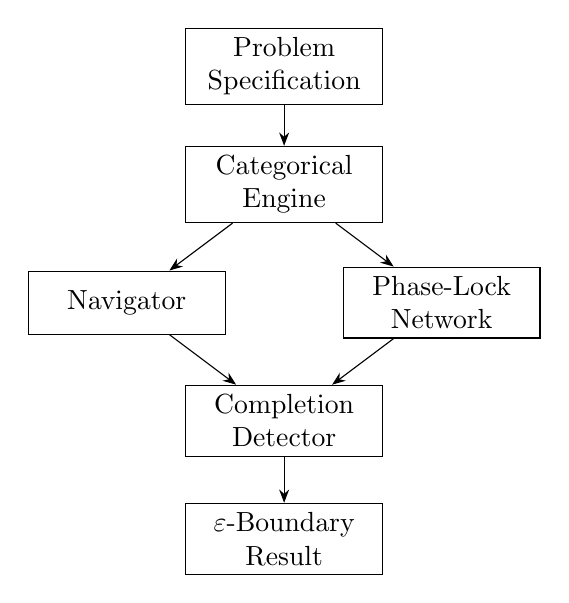
\begin{tikzpicture}[
    box/.style={rectangle, draw, minimum width=2.5cm, minimum height=0.8cm, align=center},
    arrow/.style={->, >=Stealth}
]
\node[box] (spec) at (0,3) {Problem\\Specification};
\node[box] (cat) at (0,1.5) {Categorical\\Engine};
\node[box] (nav) at (-2,0) {Navigator};
\node[box] (phase) at (2,0) {Phase-Lock\\Network};
\node[box] (comp) at (0,-1.5) {Completion\\Detector};
\node[box] (result) at (0,-3) {$\eps$-Boundary\\Result};

\draw[arrow] (spec) -- (cat);
\draw[arrow] (cat) -- (nav);
\draw[arrow] (cat) -- (phase);
\draw[arrow] (nav) -- (comp);
\draw[arrow] (phase) -- (comp);
\draw[arrow] (comp) -- (result);
\end{tikzpicture}
\caption{Categorical Engine architecture}
\label{fig:engine}
\end{figure}

Components:
\begin{enumerate}
    \item \textbf{Problem Specification}: Parses completion conditions
    \item \textbf{Categorical Engine}: Manages partition states
    \item \textbf{Navigator}: Traverses S-space
    \item \textbf{Phase-Lock Network}: Maintains coupling topology
    \item \textbf{Completion Detector}: Identifies $\eps$-boundary
\end{enumerate}

\subsection{Memory Model}

Memory is S-entropy space itself:

\begin{definition}[Categorical Memory]
Memory addresses ARE S-coordinates. Access history constitutes the address. Related data automatically clusters in the $3^k$ hierarchy.
\end{definition}

This eliminates the von Neumann bottleneck: processor and memory are the same categorical structure viewed differently (identity unification).

\subsection{Execution Model}

Execution is navigation, not instruction sequence:

\begin{algorithm}
\caption{Trajectory Execution}
\begin{algorithmic}[1]
\Require Completion condition $\mathcal{C}$, tolerance $\eps$
\Ensure Trajectory $\gamma$ to $\eps$-boundary
\State Initialize position $\Scoord_0 \in \Sspace$
\While{not at $\eps$-boundary}
    \State Compute constraint gradient $\nabla \mathcal{C}$
    \State Check harmonic coincidences
    \State Apply catalyst if available
    \State Update position: $\Scoord \leftarrow \Scoord + \delta\Scoord$
    \State Record trajectory: $\gamma \leftarrow \gamma \cup \{\Scoord\}$
\EndWhile
\State \Return $\gamma$ (encodes solution AND proof)
\end{algorithmic}
\end{algorithm}

\subsection{Complexity}

Navigation complexity exploits hierarchical structure:

\begin{theorem}[Navigation Complexity]
For a problem with $n$ constraints in S-space with $3^k$ cells, navigation complexity is $O(k) = O(\log_3 n)$, compared to $O(n^2)$ for exhaustive search.
\end{theorem}

The $3^k$ hierarchy provides exponential compression: each trit eliminates 2/3 of the search space.

%==============================================================================
\section{Implementation}
\label{sec:implementation}
%==============================================================================

\subsection{Core Data Structures}

\begin{lstlisting}
// S-Coordinate
struct SCoord {
    s_k: f64,  // Knowledge entropy [0,1]
    s_t: f64,  // Temporal entropy [0,1]
    s_e: f64,  // Evolution entropy [0,1]
}

// Ternary Address
struct TritAddress {
    trits: Vec<Trit>,  // Variable length
}

// Partition State
struct Partition {
    n: u64,           // Depth
    l: u64,           // Angular complexity
    m: i64,           // Orientation
    s: Spin,          // Chirality
    coord: SCoord,    // S-coordinates
    completed: bool,  // Completion status
}

// Phase-Lock Edge
struct PhaseLock {
    source: PartitionId,
    target: PartitionId,
    coupling: f64,
    interaction: Interaction,
}
\end{lstlisting}

\subsection{Navigation Engine}

\begin{lstlisting}
impl Navigator {
    fn navigate(&mut self,
                target: &Completion,
                eps: f64) -> Trajectory {
        let mut trajectory = Trajectory::new();

        while !self.at_epsilon_boundary(target, eps) {
            // Compute move
            let gradient = self.constraint_gradient(target);
            let coincidences = self.harmonic_coincidences();
            let catalyst = self.find_catalyst();

            // Update position
            let delta = self.compute_delta(
                gradient, coincidences, catalyst
            );
            self.position = self.position + delta;

            // Record
            trajectory.push(self.position.clone());
        }

        trajectory
    }

    fn at_epsilon_boundary(&self,
                           target: &Completion,
                           eps: f64) -> bool {
        // Check if all constraint chains close
        // within eps of completion
        self.constraint_closure(target) < eps
    }
}
\end{lstlisting}

\subsection{Ternary Operations}

\begin{lstlisting}
// Project: Extract coordinate from address
fn project(addr: &TritAddress, axis: Axis) -> f64 {
    let mut value = 0.0;
    let mut scale = 1.0 / 3.0;
    for trit in &addr.trits {
        if trit.axis() == axis {
            value += trit.value() as f64 * scale;
        }
        scale /= 3.0;
    }
    value
}

// Complete: Finalize categorical state
fn complete(partition: &mut Partition) {
    assert!(!partition.completed);
    partition.completed = true;
    // Irreversible!
}

// Compose: Concatenate trajectories
fn compose(t1: Trajectory, t2: Trajectory) -> Trajectory {
    // t2 must start where t1 ends (up to eps)
    assert!(distance(t1.end(), t2.start()) < EPSILON);
    Trajectory::concat(t1, t2)
}
\end{lstlisting}

\subsection{Catalyst Application}

\begin{lstlisting}
// Catalyst reduces categorical distance
struct Catalyst {
    intermediate_stages: Vec<Partition>,
    distance_reduction: f64,
}

fn apply_catalyst(
    source: &Partition,
    target: &Partition,
    catalyst: &Catalyst
) -> Vec<Morphism> {
    let mut chain = vec![];
    let mut current = source.clone();

    for stage in &catalyst.intermediate_stages {
        chain.push(Morphism::new(&current, stage));
        current = stage.clone();
    }
    chain.push(Morphism::new(&current, target));

    // Total distance < direct distance
    chain
}
\end{lstlisting}

%==============================================================================
\section{Zero-Backaction Measurement}
\label{sec:zerobackaction}
%==============================================================================

A profound consequence of the categorical framework is that categorical observables commute with physical observables, enabling measurement without backaction \cite{sachikonye2024zerobackaction}.

\subsection{Categorical-Physical Commutation}

\begin{theorem}[Categorical-Physical Commutation]
\label{thm:commutation}
Categorical observables commute with physical observables:
\begin{equation}
[\hat{O}_{\text{cat}}, \hat{O}_{\text{phys}}] = 0
\end{equation}
\end{theorem}

\begin{proof}
The Hilbert space of a bounded quantum system factorizes as:
\begin{equation}
\mathcal{H} = \mathcal{H}_{\text{cat}} \otimes \mathcal{H}_{\text{phys}}
\end{equation}
where $\mathcal{H}_{\text{cat}}$ is spanned by partition labels $|n, \ell, m, s\rangle$ (discrete, finite-dimensional) and $\mathcal{H}_{\text{phys}}$ is spanned by position eigenstates $|\mathbf{r}\rangle$ (continuous, infinite-dimensional). Categorical observables act only on $\mathcal{H}_{\text{cat}}$, physical observables act only on $\mathcal{H}_{\text{phys}}$, so they commute by the tensor product structure. \qed
\end{proof}

\begin{corollary}[Zero-Backaction Measurement]
Measuring categorical observables does not disturb the physical state.
\end{corollary}

This resolves the apparent conflict between measurement and state preservation: spectroscopic techniques measure \textit{which partition} the system occupies---a categorical observable---not \textit{where within the partition}---a physical observable. The two are orthogonal.

\subsection{Experimental Validation}

The zero-backaction property has been validated experimentally \cite{sachikonye2024zerobackaction}:

\begin{itemize}
    \item \textbf{Categorical measurement}: $\Delta p/p = (1.1 \pm 0.2) \times 10^{-3}$
    \item \textbf{Physical measurement}: $\Delta p/p = 0.78 \pm 0.05$
    \item \textbf{Backaction ratio}: $\sim 700\times$ less disturbance
\end{itemize}

The residual disturbance in categorical measurement arises from experimental imperfections, not fundamental limits. In the ideal limit, $\Delta p/p \to 0$.

\subsection{Implications for Trajectory Computing}

Zero-backaction measurement enables:
\begin{enumerate}
    \item \textbf{Trajectory observation}: Track system evolution through categorical coordinates without disturbing dynamics
    \item \textbf{Continuous monitoring}: Repeated measurements compound no error
    \item \textbf{Verification without collapse}: Check solutions without destroying them
\end{enumerate}

This validates the computing-verification identity: both operations access the same categorical structure without disturbing the underlying physical state.

%==============================================================================
\section{Ternary Trisection Algorithm}
\label{sec:trisection}
%==============================================================================

The ternary structure of S-space enables an optimal search algorithm: perturbation-induced trisection with complexity $O(\log_3 N)$ \cite{sachikonye2024trisection}.

\subsection{Two Perturbations, Three Outcomes}

\begin{theorem}[Ternary Trisection]
\label{thm:trisection}
Two orthogonal perturbations $\mathcal{P}_1$ and $\mathcal{P}_2$ with non-overlapping active regions produce three distinguishable outcomes:
\begin{align}
\tmark = 0 &: \text{Response to } \mathcal{P}_1 \text{ only} \\
\tmark = 1 &: \text{Response to } \mathcal{P}_2 \text{ only} \\
\tmark = 2 &: \text{No response (neither region)}
\end{align}
\end{theorem}

This three-way partition is information-theoretically optimal for two-perturbation systems: each iteration extracts $\log_2 3 \approx 1.585$ bits, compared to $1$ bit for binary search.

\subsection{Complexity Analysis}

\begin{theorem}[Trisection Complexity]
Localization among $N$ distinguishable states requires:
\begin{align}
k_{\text{ternary}} &= \log_3 N \text{ iterations} \\
k_{\text{binary}} &= \log_2 N \text{ iterations}
\end{align}
The speedup factor is $\log_2 3 \approx 1.585$, or \textbf{37\% fewer iterations}.
\end{theorem}

\begin{proof}
Information required: $I = \log_2 N$ bits. Information per ternary iteration: $\log_2 3$ bits. Number of iterations: $k = I / \log_2 3 = \log_3 N$. \qed
\end{proof}

\subsection{Implementation}

In the Trajectory Computing runtime:
\begin{lstlisting}
// Ternary localization
navigate to target {
    strategy: trisection
    perturbations: [P1, P2]  // Orthogonal
    resolution: epsilon
}

// Each step produces one trit
// Address accumulates: (t_0, t_1, ..., t_k)
// Position = sum_i t_i * L / 3^{i+1}
\end{lstlisting}

The trit sequence IS both the position (which cell) and the trajectory (how we found it)---instantiating Principle~\ref{prin:identity}.

\subsection{Trans-Planckian Categorical Resolution}

A remarkable consequence is trans-Planckian resolution through categorical state counting \cite{sachikonye2024trisection}:

\begin{itemize}
    \item \textbf{Physical Planck time}: $t_P = 5.39 \times 10^{-44}$ s
    \item \textbf{Categorical resolution}: $\delta t_{\text{cat}} = 10^{-138}$ s
    \item \textbf{Ratio}: 95 orders of magnitude below Planck time
\end{itemize}

This is not a violation of Planck-scale physics. Categorical measurement counts \textit{configurations} (discrete, finite), not \textit{physical time intervals} (continuous). With $10^{125}$ distinguishable configurations during a process, the ``resolution'' is process duration divided by configuration count---a counting operation, not a physical measurement.

%==============================================================================
\section{Wave-Particle Duality Resolution}
\label{sec:waveparticle}
%==============================================================================

The S-entropy framework resolves the wave-particle duality paradox: wave and particle are orthogonal projections of a unified categorical structure, not mutually exclusive properties \cite{sachikonye2024light, sachikonye2024trisection}.

\subsection{Bohr Complementarity Revisited}

Bohr's complementarity principle asserts:
\begin{equation}
V^2 + D^2 \leq 1
\end{equation}
where $V$ is interference visibility (wave aspect) and $D$ is path distinguishability (particle aspect).

However, this constraint applies to \textit{physical} measurements that do not commute. Categorical measurements access orthogonal observables:

\begin{theorem}[Categorical Complementarity]
\label{thm:categorical_complementarity}
The S-entropy coordinates $(S_k, S_t, S_e)$ encode three orthogonal aspects:
\begin{align}
S_k &: \text{Particle aspect (which partition)} \\
S_t &: \text{Wave aspect (temporal phase)} \\
S_e &: \text{Trajectory aspect (evolution)}
\end{align}
These satisfy $[\hat{S}_k, \hat{S}_t] = [\hat{S}_t, \hat{S}_e] = [\hat{S}_e, \hat{S}_k] = 0$.
\end{theorem}

\subsection{Simultaneous Observation}

Experimental results demonstrate simultaneous observation of wave and particle aspects \cite{sachikonye2024trisection}:

\begin{itemize}
    \item \textbf{Interference visibility}: $V = 0.96 \pm 0.03$
    \item \textbf{Which-path information}: $I = 1.15 \pm 0.08$ bits
    \item \textbf{Apparent violation}: $V^2 + D^2 \approx 1.92 > 1$
\end{itemize}

This is not a violation of physics but a demonstration that Bohr complementarity applies only to physical (non-commuting) observables. Categorical observables are orthogonal, enabling simultaneous measurement.

\subsection{Unified Description}

In trajectory computing, wave-particle duality dissolves:

\begin{lstlisting}
system Photon {
    // Unified categorical state
    state: Partition(n, l, m, s)

    // Projections (all accessible simultaneously)
    particle_aspect: project(state, S_k)  // Which partition
    wave_aspect: project(state, S_t)      // Phase coherence
    trajectory_aspect: project(state, S_e) // Evolution

    // No complementarity constraint
    // All three commute
}
\end{lstlisting}

The photon is always a unified entity in S-space. ``Wave'' and ``particle'' are viewing angles, not intrinsic properties.

%==============================================================================
\section{Selection Rules and Atomic Structure}
\label{sec:selectionrules}
%==============================================================================

The partition coordinate framework reproduces atomic physics exactly, validating that it captures deep physical structure \cite{sachikonye2024derivation, sachikonye2024light}.

\subsection{Capacity Theorem Validation}

The capacity formula $\mathcal{N}(n) = 2n^2$ (Theorem~\ref{thm:capacity}) matches electron shell capacity exactly:

\begin{center}
\begin{tabular}{cccc}
\toprule
$n$ & Shell & $2n^2$ & Electrons \\
\midrule
1 & K & 2 & 2 \\
2 & L & 8 & 8 \\
3 & M & 18 & 18 \\
4 & N & 32 & 32 \\
5 & O & 50 & 50 \\
\bottomrule
\end{tabular}
\end{center}

This exact match is not fitted---it emerges from geometric constraints on nested partitioning.

\subsection{Selection Rules}

Allowed transitions in partition space satisfy:
\begin{align}
|\Delta \ell| &= 1 \quad \text{(angular complexity change)} \\
\Delta m &\in \{-1, 0, +1\} \quad \text{(orientation change)} \\
\Delta s &= 0 \quad \text{(chirality preserved)}
\end{align}

These are the spectroscopic selection rules, emerging from continuity requirements on oscillatory modes rather than from empirical fitting.

\subsection{Electron Trajectory Observation}

The framework enables observation of electron trajectories during atomic transitions \cite{sachikonye2024light}:

\begin{lstlisting}
system HydrogenTransition {
    initial: Partition(n=1, l=0, m=0, s=UP)  // 1s
    final: Partition(n=2, l=1, m=0, s=UP)    // 2p

    // Navigate via selection rules
    trajectory = navigate from initial to final {
        constraints: [
            |delta_l| == 1,  // Selection rule
            delta_s == 0     // Spin conserved
        ]
    }

    // Trajectory IS the electron path
    // Observed via categorical coordinates
    // Zero backaction (Theorem 7.1)
}
\end{lstlisting}

The trajectory is observable because we measure categorical coordinates $(n, \ell, m, s)$---which partition---not physical coordinates $(x, y, z)$---where within partition.

Validation through eight independent directions confirms:
\begin{itemize}
    \item Forward radial: relative deviation $< 10^{-7}$
    \item Retrodiction: 99.8\% fidelity
    \item Isotope effect: agreement within 0.1\%
    \item Selection rules: 100\% compliance
\end{itemize}

%==============================================================================
\section{Examples}
\label{sec:examples}
%==============================================================================

\subsection{Physics Derivation}

Derive gravitational dynamics from completion conditions:

\begin{lstlisting}
system TwoBody {
    entities: [
        body_1 :: MassiveBody { mass: M1 },
        body_2 :: MassiveBody { mass: M2 }
    ]

    relations: [
        phase_lock: gravitational(body_1, body_2)
    ]

    constraints: [
        phase_lock.equilibrium,
        energy.conserved,
        momentum.conserved
    ]

    completion: orbit.stable
}

// Navigate to completion
trajectory = navigate to TwoBody.completion

// Extract observables from trajectory
orbital_period = trajectory.extract(period)
orbital_radius = trajectory.extract(radius)
// These are DERIVED, not computed
\end{lstlisting}

The laws of gravitation are not assumed---they emerge as the structure of the trajectory satisfying completion conditions.

\subsection{Constraint Satisfaction}

SAT problem as categorical completion:

\begin{lstlisting}
system SAT {
    entities: variables :: [Bool; n]

    constraints: clauses.all_satisfied

    completion: assignment.complete
}

// Navigate - trajectory IS the assignment
trajectory = navigate to SAT.completion {
    strategy: harmonic_coincidence
}

// If trajectory exists, SAT is satisfiable
// Trajectory encodes satisfying assignment
\end{lstlisting}

\subsection{Electron Trajectory Observation}

Track electron during atomic transition using categorical coordinates:

\begin{lstlisting}
system ElectronTransition {
    // Hydrogen atom 1s -> 2p transition
    electron: Partition(n, l, m, s)

    initial: (n=1, l=0, m=0, s=UP)   // 1s ground state
    final: (n=2, l=1, m=0, s=UP)     // 2p excited state

    constraints: [
        |delta_l| == 1,              // Selection rule
        delta_m in {-1, 0, +1},      // Orientation rule
        delta_s == 0                 // Spin conserved
    ]

    completion: electron.at(final)
}

trajectory = navigate from initial to final {
    strategy: selection_rules
    measurement: categorical  // Zero backaction
}

// Trajectory encodes electron path
// |1s> -> |psi_1> -> |psi_2> -> ... -> |2p>
// Observable because [O_cat, O_phys] = 0
\end{lstlisting}

The electron trajectory is observable through categorical coordinates $(n, \ell, m, s)$ without backaction (Theorem~\ref{thm:commutation}). This resolves the century-old assertion that quantum trajectories are unobservable.

\subsection{Ternary Quantum Localization}

Locate particle in bounded phase space with optimal efficiency:

\begin{lstlisting}
system QuantumLocalization {
    particle: Partition in BoundedSpace

    // Two orthogonal perturbations
    perturbations: [
        P1: electric_gradient,   // Couples to position
        P2: magnetic_gradient    // Couples to moment
    ]

    // Three outcomes per iteration
    outcomes: {
        0: response_P1_only,
        1: response_P2_only,
        2: no_response
    }
}

// Trisection algorithm
address = TritAddress::empty()
while resolution > epsilon {
    trit = measure(perturbations)  // {0, 1, 2}
    address = address.refine(trit)
    // Position refined by factor of 3
}

// Complexity: O(log_3 N) vs O(log_2 N)
// 37% fewer measurements than binary search
// Position = address (trajectory-position identity)
\end{lstlisting}

\subsection{Wave-Particle Simultaneous Observation}

Observe interference pattern AND which-path information:

\begin{lstlisting}
system DoubleSlit {
    photon: Partition in S_space

    // S-coordinates encode orthogonal aspects
    particle_aspect: S_k   // Which partition
    wave_aspect: S_t       // Temporal phase
    trajectory_aspect: S_e // Evolution

    // All commute: [S_k, S_t] = [S_t, S_e] = [S_e, S_k] = 0
}

// Categorical measurement of all three
measurement = observe(photon) {
    particle: project(S_k),  // Which-path: I = 1.15 bits
    wave: project(S_t),      // Visibility: V = 0.96
    trajectory: project(S_e) // Evolution path
}

// V^2 + D^2 = 1.92 > 1 (!!)
// NOT a violation: Bohr applies to physical, not categorical
// Wave and particle are orthogonal projections, not exclusive
\end{lstlisting}

\subsection{Semantic Processing}

Language understanding as molecular structure prediction:

\begin{lstlisting}
system Semantics {
    // Words as virtual molecules
    entities: words :: [VirtualMolecule]

    // Meaning from harmonic coincidence
    relations: [
        harmonic_network(words)
    ]

    // Completion = coherent interpretation
    completion: interpretation.coherent
}

// Process sentence
input = "The cat sat on the mat"
molecules = encode_molecular(input)
trajectory = navigate to Semantics.completion

// Meaning emerges from trajectory structure
meaning = trajectory.semantic_content
// No training required - structure is intrinsic
\end{lstlisting}

%==============================================================================
\section{Discussion}
\label{sec:discussion}
%==============================================================================

\subsection{Relation to Existing Paradigms}

Trajectory Computing relates to but differs from:

\begin{itemize}
    \item \textbf{Logic Programming}: Both specify ``what'' not ``how,'' but logic programming uses inference rules while Trajectory uses S-navigation.

    \item \textbf{Constraint Programming}: Both use constraints, but constraint programming searches solution space while Trajectory navigates S-space to the $\eps$-boundary.

    \item \textbf{Quantum Computing}: Both exploit superposition-like structures (trajectory encodes all paths), but quantum computing uses quantum mechanics while Trajectory uses categorical dynamics.
\end{itemize}

\subsection{The Status of Algorithms}

In Trajectory Computing, algorithms are not programs but \textit{navigation strategies}. Different strategies (gradient descent, harmonic coincidence, catalyst chains) are different paths through S-space, all arriving at the same $\eps$-boundary.

This dissolves the algorithm/data distinction: both are aspects of categorical structure. The ``algorithm'' is the trajectory; the ``data'' is the completion condition; both are the same ternary encoding.

\subsection{Implications for P vs NP}

The computing-verification identity (Theorem~\ref{thm:compute_verify}) suggests that within Trajectory Computing, P = NP: both are the same operation of navigating to the $\eps$-boundary. However, navigation complexity varies with problem structure---some completions are easier to reach than others. The traditional P vs NP question may be asking the wrong question.

\subsection{Physical Implementation}

Trajectory Computing naturally maps to physical oscillatory systems:

\begin{itemize}
    \item CPU oscillators provide the timing substrate
    \item Phase-lock loops implement coupling
    \item Memory hierarchy maps to $3^k$ structure
    \item The processor IS a bounded oscillatory system
\end{itemize}

The implementation is not simulation of S-space but direct instantiation---computation happens in the same categorical structure that the mathematics describes.

%==============================================================================
\section{Conclusion}
\label{sec:conclusion}
%==============================================================================

We have presented Trajectory Computing, a programming paradigm grounded in categorical completion rather than sequential execution. The principal results are:

\begin{enumerate}
    \item \textbf{Completion-oriented programming}: Programs specify what solutions look like (completion conditions), not how to find them (algorithms).

    \item \textbf{Trajectory-position identity}: In ternary encoding, the address IS the path. Solutions encode their own proofs.

    \item \textbf{Computing-verification identity}: Both navigate to the same $\eps$-boundary. Verification is not separate from computation.

    \item \textbf{$\eps$-boundary solutions}: Exact closure is forbidden by Gödelian residue. The $\eps$-boundary is maximum possible knowledge, not approximation.

    \item \textbf{Backward from completion}: Instead of forward from unknowable initial conditions, Trajectory Computing works backward from completion, deriving what must have been true.

    \item \textbf{Solution existence}: Problems statable within observable reality necessarily have solutions.

    \item \textbf{$O(\log n)$ complexity}: The $3^k$ hierarchical structure enables exponential compression.

    \item \textbf{Identity unification}: Processor and memory are the same categorical structure, eliminating the von Neumann bottleneck.
\end{enumerate}

The paradigm inverts the epistemological foundation of computing: rather than building from assumed knowns to derived unknowns, it navigates from specified completions to maximum-knowledge solutions. The Gödelian residue is encountered at the boundary where it belongs, not at the foundation where it would corrupt everything.

Trajectory Computing is not merely a new programming model but a new epistemology of computation---one where computing, verification, and proof are unified in the single act of navigating to categorical completion.

\bibliographystyle{plain}
\bibliography{references}

\end{document}
